% CVPR 2026 / EarthVision Workshop adaptation of the Paper 12 draft.
%
% Usage:
%   Place official CVPR style files (cvpr.sty, cvpr_eso.sty, ieeenat_fullname.bst)
%   in this directory, then compile with pdflatex+bibtex+pdflatex+pdflatex.
%   Anonymous submission: \cvprfinalcopy is commented out below.
%
% Tested target: CVPR 2026 author kit template. If submitting to the
% EarthVision workshop, replace the class options as instructed by the
% workshop call for papers.

\documentclass[10pt,twocolumn,letterpaper]{article}

\usepackage{cvpr}          % provided by CVPR author kit
\usepackage{times}
\usepackage{epsfig}
\usepackage{graphicx}
\usepackage{amsmath}
\usepackage{amssymb}
\usepackage{booktabs}
\usepackage{multirow}
\usepackage{enumitem}
\usepackage{caption}
\usepackage[breaklinks=true,bookmarks=false]{hyperref}

% Toggle for the camera-ready (de-anonymized) version.
% \cvprfinalcopy

\def\cvprPaperID{****}
\def\httilde{\mbox{\tt\raisebox{-.5ex}{\symbol{126}}}}

\ifcvprfinal\pagestyle{empty}\fi
\setcounter{page}{1}

\begin{document}

\title{How Well Do PEFT Methods Adapt Geospatial Foundation Models to Heterogeneous Inputs? A Systematic Evaluation on Prithvi-100M}

\author{Anonymous CVPR submission\\
Paper ID \cvprPaperID}

\maketitle

\begin{abstract}
Parameter-efficient fine-tuning (PEFT) is widely used to adapt large pre-trained models, but its behavior on geospatial foundation models is easily confounded by sensor mismatch, spectral-channel bridging, domain shift, and architecture-specific implementation details. This paper studies these confounders for Prithvi-100M. We evaluate seven adaptation strategies across five heterogeneous input configurations on EuroSAT, validate the main ranking on BigEarthNet-S2, extend the protocol to LandCover.ai semantic segmentation, and test whether the ranking survives a production-style Linhe County land-use/land-cover workflow and LoveDA urban/rural cross-domain transfer. The study covers 109 public-benchmark runs, a 35{,}920-patch Linhe corpus supervised by Esri-derived land-cover labels, a 30-run LoveDA cross-domain sweep, LoveDA full fine-tuning baselines, and a completed EuroSAT channel-bridge ablation comparing deterministic zero padding with a learned 10-to-6 channel projection.

The results support a diagnostic rather than universal conclusion. First, LoRA underperformance on Prithvi-100M has two separable causes: standard module-wise insertion misses the packed query, key, and value projections in fused-QKV attention, and corrected split-QKV LoRA still saturates below bottleneck adapters even when its rank is increased to a parameter budget comparable to or larger than Houlsby adapters. Second, Houlsby adapters provide the most reliable adaptation among the evaluated PEFT methods, reaching 94.5\% of the full fine-tuning score on EuroSAT s2\_full while training 1.4\% of the parameters, and widening the advantage on dense prediction. Third, input modality and domain shift strongly condition PEFT behavior: learned channel bridging improves EuroSAT accuracy while preserving the Houlsby-over-linear ordering, and LoveDA cross-domain diagnostics suggest that sub-million-parameter adapters can recover weak binary structure without recovering full multi-class semantic transfer.

These findings do not establish a universal PEFT ranking for all geospatial foundation models. They show that architecture-aware inspection, channel-bridge controls, and parameter-capacity audits are necessary before transferring PEFT intuitions from mainstream vision to Prithvi-like remote-sensing backbones. The resulting benchmark is therefore both a practical guide for Prithvi-100M deployment and a reproducible stress-test protocol for future GeoFM adaptation studies.
\end{abstract}

\section{Introduction}

Geospatial foundation models (GeoFMs) have recently emerged as a promising paradigm for Earth observation analysis. Models such as Prithvi-100M~\cite{jakubik2023prithvi}, SatMAE~\cite{cong2022satmae}, Scale-MAE~\cite{reed2023scalemae}, and related self-supervised transformers~\cite{hong2024spectralgpt} suggest that large-scale pre-training on satellite imagery can yield transferable representations for downstream remote sensing tasks. At the same time, practitioners increasingly face adaptation problems that differ substantially from the homogeneous settings used during pre-training. Real-world inputs may contain different band subsets, missing channels, alternative sensor combinations, or strongly out-of-distribution modality configurations.

In mainstream natural language processing and computer vision, parameter-efficient fine-tuning (PEFT) methods are widely used to adapt large pre-trained models at low cost. LoRA~\cite{hu2022lora}, adapters~\cite{houlsby2019adapter}, BitFit~\cite{zaken2022bitfit}, and prompt-style tuning methods~\cite{lester2021prompt,jia2022vpt} have become standard choices because they often approach full fine-tuning performance with far fewer trainable parameters. This success naturally raises the question of whether the same PEFT rankings hold for geospatial foundation models.

We argue that this assumption is non-trivial for at least three reasons. First, geospatial foundation models often operate on heterogeneous multi-band inputs rather than fixed RGB inputs. Second, remote sensing pre-training objectives, especially masked autoencoding on spectral-spatial data, differ from the language modeling and image classification setups where PEFT methods are most established. Third, implementation details that are harmless in conventional vision backbones can become critical in GeoFMs, especially when architectural components such as fused attention projections interact with adaptation layers.

Despite the practical importance of this problem, current literature lacks a systematic benchmark of PEFT methods under heterogeneous geospatial input settings. Existing studies often evaluate only one or two adaptation strategies, focus on a single downstream task, or treat PEFT as an implementation detail rather than the object of study. As a result, practitioners still lack clear guidance on which PEFT method to choose when adapting a model such as Prithvi-100M to non-standard remote sensing inputs.

A second, related gap is that PEFT comparisons are almost always reported on curated public datasets. It is rarely demonstrated that the same ranking reproduces on operational GIS pipelines, where imagery is heterogeneous in sensor and resolution, labels are derived from third-party products of varying quality, and validation splits must respect spatial structure to prevent leakage. The absence of such a demonstration is a real obstacle for practitioners deciding whether to ship a PEFT-adapted GeoFM into a production workflow. A third gap, complementary to the first two, is that within-domain PEFT comparisons cannot tell a practitioner what to expect when the target domain drifts substantially from pretraining. Cross-domain protocols on remote-sensing benchmarks --- where train and test are drawn from explicitly disjoint imaging conditions, geographies, or sensor families --- are routine in the dataset literature but largely unstudied for PEFT method ranking on geospatial foundation models.

This paper addresses all three gaps through a controlled empirical study on Prithvi-100M, paired with a production-style validation and a public cross-domain replication. We benchmark seven adaptation strategies across five modality configurations on EuroSAT, validate the main findings on BigEarthNet-S2, extend the protocol to semantic segmentation on LandCover.ai, re-instantiate the resulting five-method comparison on a 35{,}920-patch Linhe County corpus collected from 203 Chinese-domestic high-resolution scenes (0.42--4.29\,m GSD, 22 satellite families) with Esri 2022 global LULC used as supervisory labels, and finally replicate the same five-method protocol on the LoveDA urban/rural cross-domain benchmark. Beyond reporting final scores, we include a full fine-tuning ceiling, a diagnostic split-QKV LoRA ablation, a split-QKV rank-sensitivity audit, a completed EuroSAT channel-bridge ablation, a synthetic weak-label control on the Linhe corpus, and a per-class diagnostic on the LoveDA cross-domain split. The Linhe control is not an independent manual validation set; it tests whether the measured adapter delta changes when the same imagery is paired with a deliberately simple weak label. Across these experiments, we show that PEFT rankings commonly assumed in mainstream NLP and vision should not be transferred to Prithvi-100M without architecture-aware validation. We also show that benchmark rankings can be stress-tested under a geographic-split production-style workflow, while cross-domain segmentation exposes capacity and label-source limits that are not visible in within-domain classification alone.

Our main contributions are as follows:
\begin{enumerate}[leftmargin=1.5em]
    \item We report a systematic benchmark of PEFT methods on Prithvi-100M under heterogeneous input settings, covering 109 public-benchmark experiments across EuroSAT, BigEarthNet-S2, and LandCover.ai.
    \item We separate implementation failure from post-fix capacity limits for LoRA on a fused-QKV Prithvi-100M backbone: standard module-wise insertion can miss packed attention projections, while corrected split-QKV low-rank adaptation still saturates below bottleneck adapters in the tested settings.
    \item We introduce an architecture-aware PEFT audit protocol that records trainable tensors, tests fused-attention insertion, checks channel-bridge sensitivity, and compares low-rank capacity against bottleneck-adapter capacity before interpreting negative PEFT results.
    \item We show that Houlsby adapters are the strongest method in our Prithvi-100M benchmark, achieving 94.5\% of full fine-tuning performance with only 1.4\% of the trainable parameters on EuroSAT and a $+155\%$ relative mIoU gain on dense prediction.
    \item We confirm across datasets that modality selection has a larger practical impact than PEFT selection: richer spectral inputs consistently outperform reduced-band alternatives.
    \item We provide a bounded result for standalone input-stage adaptation (GeoAdapter): it is unstable on public classification benchmarks near Prithvi's pretraining modality, but becomes useful on RGB-only production-style inputs where the modality gap is larger.
    \item We test the benchmark ranking on a Linhe County LULC workflow under a geographic scene-level split, recovering Houlsby $+0.116$ mIoU over linear probing with Esri-derived supervisory labels; we also provide a synthetic weak-label control showing that the measured PEFT delta is sensitive to label source, while noting that this is not an independent manual validation set.
    \item We replicate the five-method ranking on LoveDA urban/rural cross-domain segmentation across 30 runs and report evidence consistent with an adapter-capacity threshold under domain shift. We treat this threshold as a hypothesis supported by the present diagnostics, not as a universal rule for all GeoFMs.
    \item We release a reproducible Geo-MLOps benchmarking framework together with the AlphaEarth-System platform that orchestrates the Linhe deployment, including its data pipeline, training engine, and web dashboard.
\end{enumerate}

\section{Related Work}

\subsection{Geospatial Foundation Models}
Recent years have seen rapid growth in foundation models for Earth observation. Prithvi-100M~\cite{jakubik2023prithvi}, SatMAE~\cite{cong2022satmae}, Scale-MAE~\cite{reed2023scalemae}, and SpectralGPT~\cite{hong2024spectralgpt} all extend the masked autoencoder paradigm~\cite{he2022mae} from natural images to multi-spectral and multi-temporal satellite imagery. These models share the Vision Transformer backbone~\cite{dosovitskiy2021vit} but differ from conventional vision encoders in three important ways: they ingest multi-spectral inputs rather than RGB, they exploit large unlabeled satellite corpora through self-supervised pre-training~\cite{manas2021seco,wang2022ssl4eo}, and they must support broad variation in spatial resolution and sensor configuration. While downstream transfer results are encouraging, the question of \emph{how} to adapt such models efficiently to new sensor combinations has received much less attention than the pre-training itself.

\subsection{Parameter-Efficient Fine-Tuning}
Parameter-efficient fine-tuning (PEFT) has become the standard recipe for adapting large pre-trained models without updating all parameters. BitFit~\cite{zaken2022bitfit} restricts learning to bias terms; LoRA~\cite{hu2022lora} injects low-rank updates into linear projections; Houlsby adapters~\cite{houlsby2019adapter} insert bottleneck modules between transformer blocks; and prompt-based methods~\cite{lester2021prompt,jia2022vpt} prepend learnable tokens to the input. Subsequent work has unified these strategies under a common framework~\cite{he2022unified} and explored composition across tasks~\cite{pfeiffer2020adapterfusion}. In language models and conventional vision transformers, these methods often approach full fine-tuning while reducing memory and storage costs by one to three orders of magnitude. However, their relative ranking depends strongly on architecture, task, and pre-training objective, which raises the possibility that PEFT rankings established in mainstream domains may not transfer to geospatial models.

\subsection{PEFT for Remote Sensing}
Although remote sensing research increasingly relies on pre-trained transformers, systematic evaluation of PEFT methods in this domain remains limited. Existing work tends to focus on a single adaptation method, a single dataset, or an application-specific pipeline; PEFT is typically adopted pragmatically rather than studied comparatively. Closely related lines of work, such as training-free adaptation in vision-language models~\cite{zhang2022tip}, show that adaptation strategy can dominate over backbone choice, but this observation has not been verified for geospatial foundation models. As a result, the field still lacks a controlled benchmark answering basic but practically important questions: Does LoRA~\cite{hu2022lora} work as expected on geospatial transformers? Which adapter family is most robust under heterogeneous input configurations? How much of the gap to full fine-tuning can be closed under small parameter budgets? Our work is designed to answer these questions directly.

\section{Experimental Setup}

\subsection{Foundation Model}
We use Prithvi-100M~\cite{jakubik2023prithvi} as the shared backbone in all experiments. Prithvi-100M is an 86M-parameter Vision Transformer~\cite{dosovitskiy2021vit} pre-trained on remote sensing imagery using a masked autoencoding objective~\cite{he2022mae}. In our implementation, the backbone consists of a 12-layer transformer encoder with embedding dimension 768, 12 attention heads, and an input patch embedding layer adapted for six expected input channels. Unless otherwise noted, the backbone is frozen and only PEFT parameters and task heads are updated.

A key architectural detail is that Prithvi's attention uses a fused QKV projection pattern inherited through PyTorch's \texttt{nn.MultiheadAttention}, where query, key, and value weights are stored as a single \texttt{in\_proj\_weight} parameter. This detail turns out to be crucial for interpreting LoRA results.

\subsection{PEFT Methods}
We evaluate seven adaptation strategies:
\begin{itemize}[leftmargin=1.5em]
    \item \textbf{Linear Probe}: frozen backbone with a trainable classification head.
    \item \textbf{BitFit}~\cite{zaken2022bitfit}: unfreezes only bias parameters throughout the backbone.
    \item \textbf{LoRA (r=8)}~\cite{hu2022lora}: standard low-rank adaptation inserted into attention projections.
    \item \textbf{LoRA Split-QKV (r=8)}: diagnostic variant that explicitly splits fused QKV into separate query, key, and value linear layers before injecting LoRA.
    \item \textbf{Houlsby Adapters (d=64)}~\cite{houlsby2019adapter}: bottleneck adapters inserted after each transformer block.
    \item \textbf{GeoAdapter v2}: residual input-stage modality adapter.
    \item \textbf{Full Fine-Tuning}: unfreezes all backbone parameters (EuroSAT only) to establish the performance ceiling.
\end{itemize}

The trainable parameter counts range from 7.7K for EuroSAT linear probing to 86.2M for full fine-tuning.

\subsection{Modality Configurations}
We define five input configurations on EuroSAT to stress-test adaptation under heterogeneous spectral settings:
\begin{itemize}[leftmargin=1.5em]
    \item \textbf{s2\_full}: all 10 Sentinel-2 bands (B2--B12).
    \item \textbf{rgb}: visible subset (B4, B3, B2).
    \item \textbf{rgb\_sar}: RGB plus a simulated extra channel.
    \item \textbf{gf2}: a 4-band high-resolution optical proxy (B, G, R, NIR).
    \item \textbf{sar\_only}: 2-band extreme out-of-distribution configuration.
\end{itemize}

Because Prithvi expects six channels, all non-matching inputs are bridged either by the deterministic \texttt{ZeroPadAdapter} or by GeoAdapter. \texttt{ZeroPadAdapter} pads missing channels with zeros when $c_{\mathrm{in}}<6$ and truncates excess selected channels when $c_{\mathrm{in}}>6$. The zero-padding/truncation setup is not merely a preprocessing trick; it is part of the evaluation, since it reveals whether different PEFT methods can exploit partially missing or mismatched channels. This design also defines the boundary of the present results: the \texttt{s2\_full} preset uses selected Sentinel-2 channels before the six-channel Prithvi bridge, not a newly trained 10-channel patch embedding.

For BigEarthNet-S2, we evaluate two configurations: \texttt{s2\_full} and \texttt{rgb}. This is sufficient to test whether the main EuroSAT conclusions transfer to a second dataset and a multi-label task.

\subsection{Datasets}
\textbf{EuroSAT}~\cite{helber2019eurosat} is used as the primary benchmark. It contains 27K Sentinel-2 image patches at 64\,$\times$\,64 resolution across 10 land-use classes. We use three random seeds and report mean and standard deviation across runs.

\textbf{BigEarthNet-S2}~\cite{sumbul2019bigearthnet} is used for cross-dataset validation. To keep experiments tractable on Colab A100 hardware, we use a 10K/5K train/validation subsample from the 19-class simplified multi-label setting. Evaluation uses mean Average Precision (mAP).

\subsection{Training Protocol}
All experiments are run on Google Colab Pro+ with an NVIDIA A100 40GB GPU. EuroSAT experiments use 50 epochs; BigEarthNet experiments use 15 epochs. The optimizer is AdamW~\cite{loshchilov2019adamw} with cosine annealing~\cite{loshchilov2017sgdr}. We use a batch size of 64 in standard PEFT runs, and batch size 32 for full fine-tuning to avoid memory overflow. Differential learning rates are used where appropriate: PEFT parameters receive a lower learning rate than the task head.

For EuroSAT, we report Overall Accuracy (OA) and macro F1. For BigEarthNet-S2, we report mAP. Results are aggregated over three seeds whenever possible; the full fine-tuning ceiling is reported as a single run.

\subsection{Evaluation Boundary}
The experiments are designed to test PEFT behavior for Prithvi-100M rather than to establish a universal ranking for all geospatial foundation models. The study therefore makes three bounded claims. First, the fused-QKV LoRA failure is an implementation risk for Prithvi-like PyTorch attention modules, not a proof that LoRA is ineffective on every remote sensing backbone. Second, the Houlsby advantage is established under the parameter budgets and datasets reported here, and the completed capacity sweep now shows that the EuroSAT gap is not explained by LoRA having fewer trainable parameters alone. Third, the Linhe labels are derived from an external land-cover product and should be interpreted as production-style supervisory labels rather than manually annotated ground truth.

\subsection{Completed EuroSAT Capacity-Audit Extension}
To address the parameter-budget confound directly, we completed a 30-run EuroSAT capacity sweep without changing the training framework. The audit uses EuroSAT s2\_full, the same Prithvi-100M checkpoint, the same seeds $\{42,123,456\}$, and the same OA/macro-F1 metrics. It compares split-QKV LoRA ranks $r\in\{4,8,16,32,64\}$ against Houlsby bottleneck widths $d\in\{8,16,32,64\}$, with linear probing as the frozen-backbone floor. The Colab notebook and config are released as \texttt{colab/paper12\_peft\_capacity\_sweep\_colab.ipynb} and \texttt{geoadapter/bench/configs/eurosat\_peft\_capacity\_sweep.yaml}; the raw and summarized outputs are released as \texttt{paper12\_results/peft\_capacity\_sweep.json} and \texttt{paper12\_results/peft\_capacity\_sweep\_summary.json}. This audit separates adapter placement from parameter count in the tested Prithvi-100M/EuroSAT setting. To make the reviewer-facing checks reproducible, we also release a derived audit file, \texttt{paper12\_results/review\_audit\_summary.json}, generated by \texttt{python -m geoadapter.bench.paper12\_audit}. It reads the completed capacity-sweep, channel-bridge, LoveDA PEFT, LoveDA full-finetuning, LoveDA diagnostic, LandCover.ai segmentation, and Linhe LULC artifacts, and records the exact capacity, ordering, model-scope, label-source, and decoder-capacity checks used to bound the Discussion.

\section{Results and Analysis}

\subsection{Main EuroSAT Results}
Table~\ref{tab:eurosat-main} reports overall accuracy across all five modality configurations on EuroSAT. Houlsby adapters dominate every modality, while standard LoRA tracks the linear-probe baseline within $\pm 0.001$ OA --- consistent with complete failure under the original implementation. The split-QKV ablation recovers most of LoRA's expected gain on s2\_full but, as analyzed below, still falls short of both BitFit and Houlsby.

\begin{table}[t]
\centering
\small
\caption{EuroSAT~\cite{helber2019eurosat} overall accuracy across five modality configurations. Mean $\pm$ std over three seeds; full fine-tuning is reported as a single run. Best PEFT result per column in \textbf{bold}.}
\label{tab:eurosat-main}
\begin{tabular}{lccccc}
\toprule
Method & s2\_full & rgb & rgb\_sar & gf2 & sar\_only \\
\midrule
Linear Probe        & 0.657 $\pm$ 0.002 & 0.556 $\pm$ 0.004 & 0.552 $\pm$ 0.002 & 0.649 $\pm$ 0.006 & 0.387 $\pm$ 0.004 \\
BitFit              & 0.702 $\pm$ 0.002 & 0.608 $\pm$ 0.001 & 0.605 $\pm$ 0.002 & 0.701 $\pm$ 0.001 & 0.449 $\pm$ 0.003 \\
LoRA (r=8)          & 0.658 $\pm$ 0.003 & 0.556 $\pm$ 0.003 & 0.553 $\pm$ 0.003 & 0.650 $\pm$ 0.006 & 0.388 $\pm$ 0.004 \\
LoRA Split-QKV      & 0.707 $\pm$ 0.003 & 0.498 $\pm$ 0.006 & --- & --- & --- \\
Houlsby             & \textbf{0.821 $\pm$ 0.003} & \textbf{0.727 $\pm$ 0.003} & \textbf{0.738 $\pm$ 0.002} & \textbf{0.820 $\pm$ 0.002} & \textbf{0.615 $\pm$ 0.004} \\
GeoAdapter v2       & 0.485 $\pm$ 0.056 & 0.383 $\pm$ 0.015 & --- & --- & --- \\
\midrule
Full Fine-Tuning    & 0.869 & --- & --- & --- & --- \\
\bottomrule
\end{tabular}
\end{table}

Two patterns are immediately visible. (i)~The Houlsby--linear-probe gap is consistent across modalities ($+16.4\%$ to $+22.8\%$ OA), suggesting the gain is structural rather than modality-specific. (ii)~The cross-modality gap dominates the cross-method gap whenever the spectral input is degraded: switching from s2\_full to sar\_only costs more accuracy (e.g.~$-20.6\%$ for Houlsby) than switching between PEFT methods at fixed modality.

\subsection{Main BigEarthNet Results}
Table~\ref{tab:bigearthnet-main} validates the EuroSAT ranking on a larger, multi-label benchmark. Houlsby again leads, while LoRA and linear probing are statistically indistinguishable.

\begin{table}[t]
\centering
\caption{BigEarthNet-S2~\cite{sumbul2019bigearthnet} validation mAP (19-class multi-label, mean $\pm$ std over three seeds).}
\label{tab:bigearthnet-main}
\begin{tabular}{lcc}
\toprule
Method & s2\_full & rgb \\
\midrule
Linear Probe & 0.358 $\pm$ 0.003 & 0.335 $\pm$ 0.001 \\
LoRA (r=8) & 0.358 $\pm$ 0.003 & 0.335 $\pm$ 0.001 \\
Houlsby & \textbf{0.491 $\pm$ 0.008} & \textbf{0.456 $\pm$ 0.003} \\
\bottomrule
\end{tabular}
\end{table}

\subsection{Finding 1: Why LoRA Fails}
The naive LoRA result initially suggested complete failure: on EuroSAT, LoRA differs from linear probing by only $+0.001$ OA, and on BigEarthNet-S2 by only $+0.0001$ mAP. Our split-QKV ablation reveals that this failure has two distinct causes.

First, the standard implementation misses the actual query, key, and value projections because Prithvi's attention stores them as a fused \texttt{in\_proj\_weight} parameter rather than as separate child modules. As a result, the original LoRA insertion only wraps \texttt{out\_proj}. Second, even when the fused QKV issue is corrected, LoRA remains suboptimal. Split-QKV LoRA improves s2\_full from 0.658 to 0.707 on EuroSAT, confirming the implementation trap is real, but it still underperforms both BitFit and Houlsby. On rgb, split-QKV LoRA actually degrades below the linear probing baseline.

Together, these observations show that LoRA fails on Prithvi-100M not only because of an implementation pitfall, but also because low-rank adaptation appears mismatched to this architecture and pre-training regime. We further validated this point with a rank-sensitivity ablation on EuroSAT s2\_full (Figure~\ref{fig:lora-rank}): increasing the split-QKV LoRA rank from $r=4$ to $r=32$ changes OA only from $0.709 \pm 0.002$ to $0.706 \pm 0.002$, with no monotonic improvement and no configuration approaching Houlsby.

\begin{figure}[t]
\centering
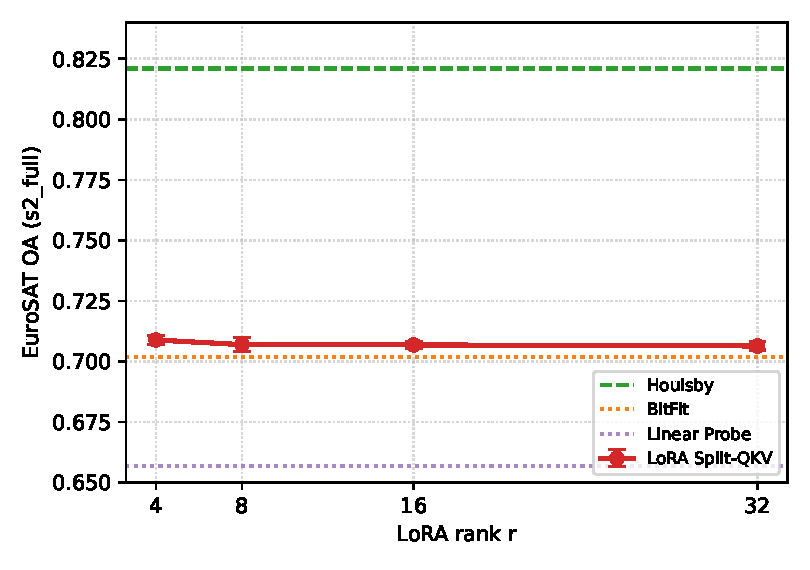
\includegraphics[width=0.78\linewidth]{figures/lora_rank_sensitivity.pdf}
\caption{Split-QKV LoRA rank sensitivity on EuroSAT s2\_full. Raising the rank from 4 to 32 does not materially improve accuracy, indicating that the post-fix LoRA ceiling is not explained by an underpowered rank choice.}
\label{fig:lora-rank}
\end{figure}

\subsection{Finding 2: Houlsby Consistently Dominates}
Houlsby adapters are the best method on every evaluated configuration. On EuroSAT, they outperform linear probing by $+16.4\%$ to $+22.8\%$ OA depending on modality. On BigEarthNet-S2, they outperform linear probing by $+13.3$ mAP on s2\_full and $+12.1$ mAP on rgb. This consistency across datasets and tasks is the strongest empirical conclusion of the benchmark. The full fine-tuning baseline further clarifies the quality of this result: full fine-tuning reaches 0.869 OA on EuroSAT s2\_full while Houlsby reaches 0.821, corresponding to 94.5\% of the full fine-tuning score with only 1.4\% of the trainable parameters (Figure~\ref{fig:acc-vs-params}).

\begin{figure}[t]
\centering
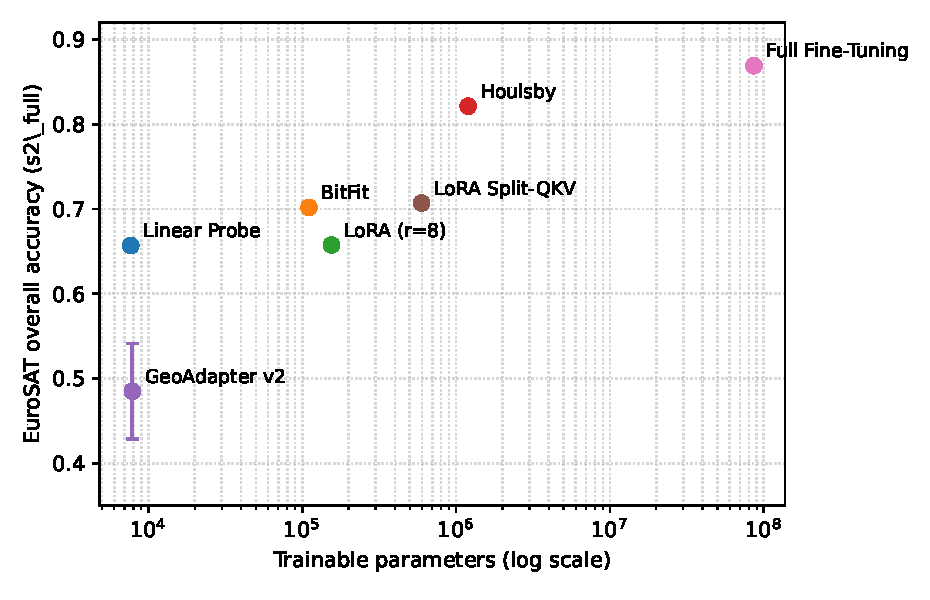
\includegraphics[width=0.78\linewidth]{figures/acc_vs_params.pdf}
\caption{EuroSAT s2\_full overall accuracy versus trainable parameter count (log scale). Houlsby adapters reach 94.5\% of the full fine-tuning ceiling using 1.4\% of the parameters; standard LoRA collapses to the linear-probe baseline.}
\label{fig:acc-vs-params}
\end{figure}

\subsection{Finding 3: Modality Selection Matters More Than Method Selection}
Across both datasets, richer spectral inputs consistently outperform reduced-band subsets. On BigEarthNet-S2, the s2\_full--rgb gap is $+0.023$ mAP for linear probing, $+0.023$ mAP for LoRA, and $+0.035$ mAP for Houlsby. On EuroSAT (Figure~\ref{fig:per-modality}), the spread between modalities is even larger: switching from s2\_full to sar\_only costs Houlsby $-20.6\%$ OA, more than the entire spread between BitFit and Houlsby on s2\_full.

\begin{figure}[t]
\centering
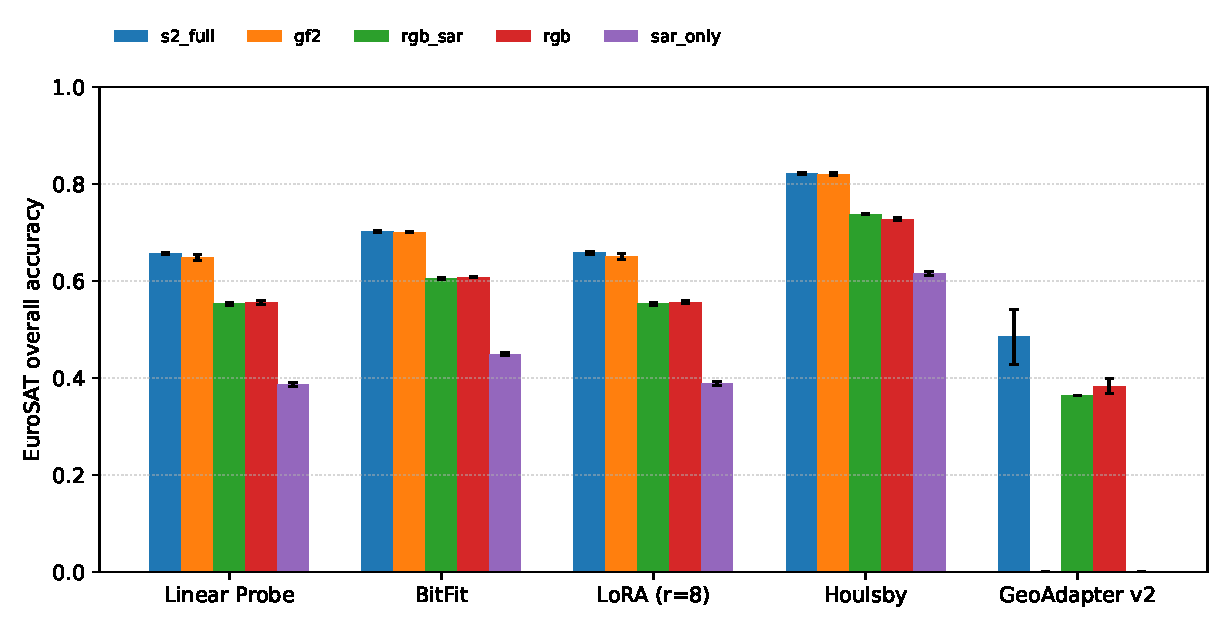
\includegraphics[width=0.92\linewidth]{figures/per_modality_oa.pdf}
\caption{EuroSAT overall accuracy per modality, grouped by PEFT method. Modality selection (color groups) shifts OA more than method selection (within-group ordering) for every method except linear probing.}
\label{fig:per-modality}
\end{figure}

This result suggests that practitioners should first maximize input information quality before worrying about subtle PEFT differences. A simple linear probe on better spectral inputs can outperform more sophisticated adaptation on weaker input subsets.

\subsection{Finding 4: Input-Stage Adaptation Remains a Negative Result}
GeoAdapter v2 consistently underperforms the linear probing baseline on EuroSAT. Although it was designed to bridge modality mismatches at the input stage, its residual adapter structure does not provide a stable optimization path under a frozen transformer backbone. The high seed variance on s2\_full ($\pm 0.056$) is itself diagnostic: the optimization landscape is unstable, and the negative result therefore reflects a structural rather than a hyperparameter issue. We conclude that modality adaptation is more effectively handled by backbone-level PEFT than by a tiny standalone input bridge.

\subsection{Practical Takeaways}
The benchmark supports three practical recommendations. First, Houlsby adapters are the safest default for adapting Prithvi-100M to heterogeneous inputs. Second, LoRA should not be assumed effective in GeoFMs without careful architectural inspection. Third, when spectral richness is available, preserving that information has larger returns than switching between weak PEFT methods.

\section{Discussion}
\label{sec:discussion}

\subsection{Why Does Low-Rank Adaptation Underperform on Prithvi?}
Our split-QKV ablation isolates two effects. The \emph{implementation trap} reflects a property of PyTorch's \texttt{nn.MultiheadAttention}, in which query, key, and value weights are packed into a single \texttt{in\_proj\_weight} tensor. A naive application of LoRA to named \texttt{nn.Linear} children therefore touches only \texttt{out\_proj}, leaving the attention projections effectively frozen. This is a silent failure mode: training proceeds, loss decreases, and accuracy settles only slightly above linear probing, which can easily be misread as a genuine negative result.

Once Q, K, and V are explicitly exposed, split-QKV LoRA improves EuroSAT s2\_full from 0.658 to 0.707 but remains below both BitFit (0.702) and Houlsby (0.821). We attribute this residual gap to two factors. First, the masked autoencoding objective~\cite{he2022mae} used by Prithvi produces features whose task-relevant directions are not well captured by low-rank updates to attention alone; richer adaptation (bottleneck MLPs) appears to be required. Second, the frozen backbone restricts LoRA to reshaping existing attention patterns, whereas Houlsby adapters introduce new non-linear capacity inside each block. This is consistent with the unified view of PEFT proposed in prior work~\cite{he2022unified}, which predicts that methods with both extra capacity and non-linearity can dominate under sufficiently different pre-training distributions. A follow-up rank-sensitivity ablation strengthens this interpretation: increasing split-QKV LoRA from $r=4$ to $r=32$ leaves EuroSAT s2\_full accuracy essentially flat at 0.706--0.709, ruling out the simple explanation that the negative result is caused by an underpowered rank choice alone.

\subsection{When Does Input-Stage Adaptation Help?}
GeoAdapter v2 places a small residual module before the patch embedding. Conceptually, this is attractive for modality bridging, but the empirical picture is regime-dependent. On EuroSAT, where the input is 13-band Sentinel-2 close to Prithvi's HLS pretraining modality, GeoAdapter underperforms linear probing on every modality configuration: the input-stage residual has limited new information to add, and the small parameter budget is insufficient to jointly learn modality alignment and useful feature transformation. On the Linhe production corpus (Section~\ref{sec:linhe}), where the input is 3-band RGB padded with zeros into the HLS template --- a substantial modality shift --- GeoAdapter recovers $+0.087$ mIoU over linear probing at only 4{,}756 parameters, second only to Houlsby's bottleneck adapters. We therefore refine the negative result: input-stage adaptation is fragile when the modality shift is small and the patch embedding is already well-tuned, but becomes useful as the input drifts further from the backbone's pretraining distribution. The recommendation is to treat GeoAdapter as a deployment-time decision: profile the modality gap first, then decide. Two underlying mechanisms still bound its potential. First, the module lies on the critical gradient path to a frozen backbone, so any early-stage misadaptation propagates unchallenged through 12 transformer blocks. Second, the adapter has no clear pre-training prior, unlike bottleneck adapters that operate on already well-structured hidden states. Future modality bridging work should combine input-stage and backbone-level adaptation rather than rely on either alone.

\subsection{Architecture-Awareness as a Methodological Principle}
The fused-QKV trap has an uncomfortable implication: published PEFT comparisons on Prithvi-like backbones may silently conflate \emph{method failure} with \emph{implementation failure}. We believe this motivates a broader methodological recommendation. Before reporting negative results for PEFT methods on any new architecture, authors should report (i) exactly which parameter tensors were registered as trainable, (ii) whether the attention projections are fused, and (iii) whether a diagnostic split variant was attempted. Our study adopts this protocol and we encourage its adoption for future GeoFM benchmarks.

\subsection{Practical Guidance and Limitations}
For practitioners adapting Prithvi-100M to heterogeneous inputs, the safest default is Houlsby adapters with bottleneck dimension 64, which reach 94.5\% of the full fine-tuning ceiling on EuroSAT s2\_full while training 1.4\% of parameters. When spectral richness is available, preserving it yields larger returns than switching between PEFT methods: a linear probe on s2\_full outperforms sophisticated adaptation on sar\_only. LoRA should not be used on fused-QKV backbones without explicit Q/K/V exposure and, even then, should be justified empirically against adapter baselines.

Our study has three limitations. First, we evaluate a single backbone, Prithvi-100M; extension to SatMAE~\cite{cong2022satmae}, Scale-MAE~\cite{reed2023scalemae}, and SpectralGPT~\cite{hong2024spectralgpt} would strengthen the generality of conclusions. Second, although we now cover classification (single-label on EuroSAT, multi-label on BigEarthNet-S2) and dense prediction (semantic segmentation on LandCover.ai), regression and temporal forecasting remain open. Third, our BigEarthNet-S2 subsample (10K/5K) is chosen for Colab-scale tractability and may under-represent the long tail of rare classes; full-scale replication is an obvious next step.

\section{Conclusion}

We presented an architecture-aware diagnosis of PEFT behavior for adapting Prithvi-100M to heterogeneous geospatial inputs. Across EuroSAT, BigEarthNet-S2, LandCover.ai, Linhe, and LoveDA, the results support a bounded conclusion: PEFT rankings familiar from NLP and conventional vision should be revalidated on remote-sensing foundation models with explicit inspection of attention implementation, input-channel bridging, trainable tensors, and domain shift. In the tested Prithvi-100M setting, Houlsby adapters provide the strongest and most reliable adaptation performance, and their advantage widens on dense prediction rather than shrinking.

The main methodological contribution is not simply that one adapter family wins a benchmark. The study separates two LoRA failure modes that would otherwise be conflated: standard module-wise insertion misses fused QKV projections, and corrected split-QKV low-rank adaptation still remains below bottleneck adapters in the tested settings even when LoRA is given a larger trainable-parameter budget. The completed channel-bridge ablation further shows that input bridging changes absolute EuroSAT accuracy but does not remove the Houlsby-over-linear ordering. The Linhe and LoveDA experiments then show why curated benchmark scores are insufficient: label provenance, geographic split, class imbalance, and cross-domain transfer can change both the absolute operating point and the amount of adapter capacity needed to recover multi-class semantic structure.

These conclusions remain deliberately bounded. We focus on one backbone, Prithvi-100M, and Linhe uses Esri-derived supervisory labels rather than independent manual ground truth. The completed EuroSAT capacity sweep supports the capacity-boundary interpretation within the tested Prithvi setting, but additional backbones are still needed before converting this into a general GeoFM rule. Despite these limits, the benchmark provides a reproducible stress-test protocol for GeoFM adaptation: inspect the architecture before injecting PEFT modules, control the channel bridge, compare capacity as well as method family, and report per-class diagnostics when domain shift is severe.


{\small
\bibliographystyle{ieeenat_fullname}
\bibliography{references}
}

\appendix

\section{Full Per-Seed Results}
\label{app:per-seed}

This appendix reports the per-seed values that underlie the aggregated tables in the main paper. All EuroSAT runs use 50 epochs; BigEarthNet-S2 runs use 15 epochs. Seeds are $\{42, 123, 456\}$ throughout.

\subsection{EuroSAT Per-Seed Overall Accuracy}

\begin{table}[h]
\centering
\small
\caption{EuroSAT per-seed overall accuracy. Each cell is a single training run.}
\label{tab:eurosat-per-seed}
\begin{tabular}{llccc}
\toprule
Method & Modality & seed=42 & seed=123 & seed=456 \\
\midrule
\multirow{5}{*}{Linear Probe}
 & s2\_full   & 0.6589 & 0.6543 & 0.6572 \\
 & rgb        & 0.5570 & 0.5594 & 0.5519 \\
 & rgb\_sar   & 0.5544 & 0.5531 & 0.5498 \\
 & gf2        & 0.6452 & 0.6457 & 0.6559 \\
 & sar\_only  & 0.3870 & 0.3833 & 0.3913 \\
\midrule
\multirow{5}{*}{BitFit}
 & s2\_full   & 0.6996 & 0.7026 & 0.7035 \\
 & rgb        & 0.6076 & 0.6089 & 0.6067 \\
 & rgb\_sar   & 0.6072 & 0.6039 & 0.6052 \\
 & gf2        & 0.7004 & 0.7019 & 0.6998 \\
 & sar\_only  & 0.4470 & 0.4480 & 0.4524 \\
\midrule
\multirow{5}{*}{LoRA (r=8)}
 & s2\_full   & 0.6604 & 0.6548 & 0.6576 \\
 & rgb        & 0.5546 & 0.5596 & 0.5546 \\
 & rgb\_sar   & 0.5557 & 0.5530 & 0.5504 \\
 & gf2        & 0.6444 & 0.6480 & 0.6563 \\
 & sar\_only  & 0.3913 & 0.3831 & 0.3900 \\
\midrule
\multirow{5}{*}{Houlsby}
 & s2\_full   & 0.8189 & 0.8207 & 0.8241 \\
 & rgb        & 0.7294 & 0.7278 & 0.7244 \\
 & rgb\_sar   & 0.7389 & 0.7361 & 0.7387 \\
 & gf2        & 0.8226 & 0.8198 & 0.8178 \\
 & sar\_only  & 0.6111 & 0.6161 & 0.6191 \\
\midrule
\multirow{2}{*}{LoRA Split-QKV}
 & s2\_full   & 0.7093 & 0.7080 & 0.7037 \\
 & rgb        & 0.4969 & 0.4922 & 0.5035 \\
\midrule
\multirow{2}{*}{GeoAdapter v2}
 & s2\_full   & 0.5494 & 0.4607 & 0.4448 \\
 & rgb        & 0.3878 & 0.3956 & 0.3659 \\
\midrule
Full Fine-Tuning & s2\_full & 0.8685 & --- & --- \\
\bottomrule
\end{tabular}
\end{table}

\subsection{BigEarthNet-S2 Per-Seed mAP}

\begin{table}[h]
\centering
\small
\caption{BigEarthNet-S2 per-seed validation mAP (19-class multi-label).}
\label{tab:bigearthnet-per-seed}
\begin{tabular}{llccc}
\toprule
Method & Modality & seed=42 & seed=123 & seed=456 \\
\midrule
\multirow{2}{*}{Linear Probe}
 & s2\_full   & 0.3578 & 0.3606 & 0.3548 \\
 & rgb        & 0.3344 & 0.3343 & 0.3363 \\
\midrule
\multirow{2}{*}{LoRA (r=8)}
 & s2\_full   & 0.3582 & 0.3606 & 0.3545 \\
 & rgb        & 0.3346 & 0.3350 & 0.3363 \\
\midrule
\multirow{2}{*}{Houlsby}
 & s2\_full   & 0.4927 & 0.4815 & 0.4979 \\
 & rgb        & 0.4531 & 0.4583 & 0.4559 \\
\bottomrule
\end{tabular}
\end{table}

\section{Trainable Parameter Budgets}
\label{app:params}

Table~\ref{tab:params} reports the exact trainable parameter count per method, isolated from the frozen Prithvi-100M backbone. The classification head accounts for 7{,}690 parameters on EuroSAT (10 classes) and 14{,}611 on BigEarthNet-S2 (19 classes).

\begin{table}[h]
\centering
\small
\caption{Trainable parameter counts (head included).}
\label{tab:params}
\begin{tabular}{lrr}
\toprule
Method & EuroSAT & BigEarthNet \\
\midrule
Linear Probe       &      7{,}690 &     14{,}611 \\
GeoAdapter v2      &      7{,}873 &        --- \\
BitFit             &    110{,}602 &        --- \\
LoRA (r=8)         &    155{,}146 &    162{,}067 \\
LoRA Split-QKV     &    597{,}514 &        --- \\
Houlsby (d=64)     &  1{,}197{,}322 &  1{,}204{,}243 \\
Full Fine-Tuning   & 86{,}244{,}874 &        --- \\
\bottomrule
\end{tabular}
\end{table}

\section{Training Curves}
\label{app:curves}

Figure~\ref{fig:curve-eurosat} compares the training loss trajectories of full fine-tuning and split-QKV LoRA on EuroSAT s2\_full. Full fine-tuning converges to a substantially lower loss, consistent with its higher final accuracy. Figure~\ref{fig:curve-ben} shows the BigEarthNet-S2 loss curves for the three methods evaluated on that dataset; Houlsby separates from the LoRA/linear-probe cluster early in training.

\begin{figure}[h]
\centering
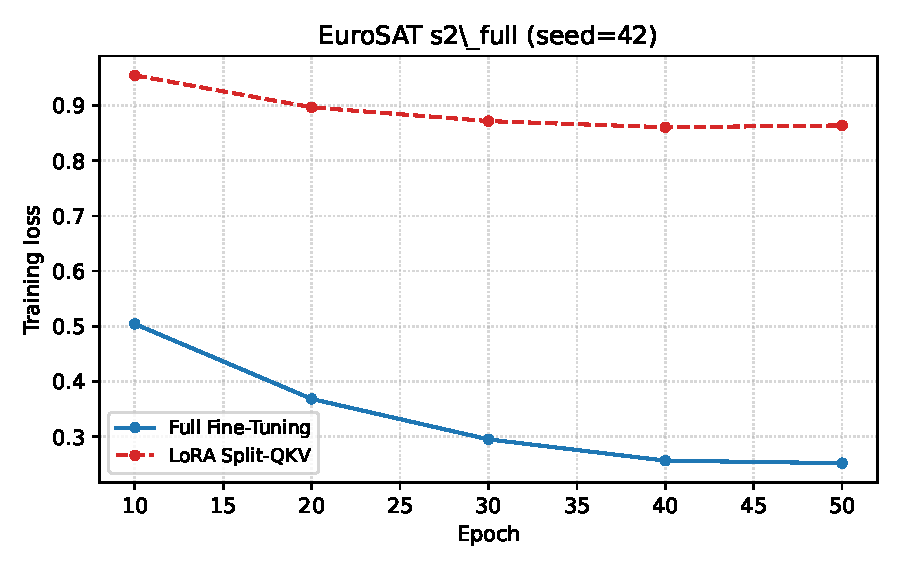
\includegraphics[width=0.85\linewidth]{figures/training_curves_eurosat.pdf}
\caption{Training loss on EuroSAT s2\_full (seed=42). Full fine-tuning reaches a much lower loss floor than split-QKV LoRA.}
\label{fig:curve-eurosat}
\end{figure}

\begin{figure}[h]
\centering
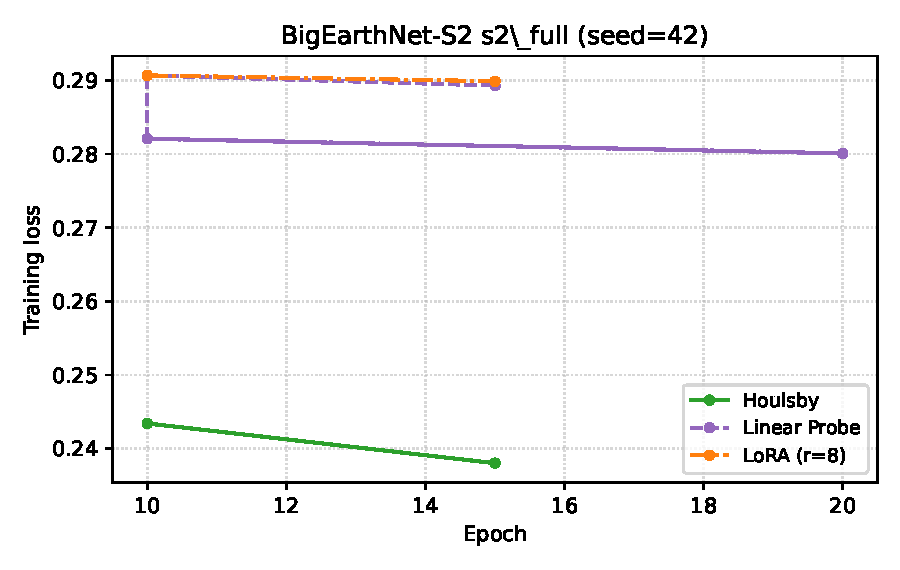
\includegraphics[width=0.85\linewidth]{figures/training_curves_bigearthnet.pdf}
\caption{Training loss on BigEarthNet-S2 s2\_full (seed=42). Houlsby separates from LoRA and linear probing by epoch 10.}
\label{fig:curve-ben}
\end{figure}

\section{Hyperparameters and Compute}
\label{app:hparams}

\paragraph{Optimizer and schedule.}
All runs use AdamW~\cite{loshchilov2019adamw} with cosine annealing~\cite{loshchilov2017sgdr}. Weight decay is $10^{-4}$. The PEFT-parameter learning rate is $10^{-3}$ on EuroSAT and $5\times 10^{-4}$ on BigEarthNet-S2; the classification head receives $5\times 10^{-3}$ throughout. Full fine-tuning uses a single learning rate of $5\times 10^{-5}$.

\paragraph{Batching.}
Standard PEFT runs use batch size 64. Full fine-tuning uses batch size 32 to fit within 40\,GB of A100 memory. BigEarthNet uses batch size 64 for all methods.

\paragraph{Compute.}
All experiments run on a single NVIDIA A100 40\,GB on Google Colab Pro+. Wall-clock time per run averages 19--23 minutes on EuroSAT and 28--34 minutes on BigEarthNet (15 epochs over the 10K subsample). Total compute for the 100 reported runs is approximately 38 GPU-hours.

\paragraph{Data preparation.}
EuroSAT patches are resized from $64\times 64$ to $224\times 224$ and standardized per-band against statistics computed on the training split. BigEarthNet patches are decoded from the GeoTIFF format, resized to $120\times 120$ and standardized identically. Channel zero-padding is applied at the dataloader level to bridge any modality with fewer than 6 channels to Prithvi's 6-channel input expectation.

\section{LoRA Rank Sensitivity}
\label{app:lora-rank}

To test whether the split-QKV LoRA result is merely limited by an underpowered rank choice, we ran an additional ablation on EuroSAT s2\_full with $r\in\{4,8,16,32\}$. The corresponding trainable parameter counts are 302{,}602, 597{,}514, 1{,}187{,}338, and 2{,}366{,}986. The mean overall accuracies (3 seeds each) are 0.7089 $\pm$ 0.0018 ($r=4$), 0.7070 $\pm$ 0.0029 ($r=8$), 0.7069 $\pm$ 0.0013 ($r=16$), and 0.7064 $\pm$ 0.0017 ($r=32$). Figure~\ref{fig:lora-rank} in the main paper visualizes this trend.

The result is qualitatively stable: increasing the LoRA rank does not produce monotonic gains and never approaches the Houlsby adapter score of 0.821. This makes the post-fix LoRA ceiling much harder to dismiss as a hyperparameter artifact. Within the explored budget range, the limitation appears architectural rather than rank-bound.

\section{LoRA Implementation Details and the Fused-QKV Trap}
\label{app:lora-trap}

This section documents the exact code-level cause of the LoRA failure observed in the main paper, since reproducing or refuting our negative result requires reproducing the same insertion pattern.

Prithvi-100M's attention block is implemented as a \texttt{torch.nn.MultiheadAttention} module. In PyTorch's reference implementation, the query, key, and value projections are stored as a single tensor:

\begin{verbatim}
attn.in_proj_weight        # shape [3*D, D]
attn.in_proj_bias          # shape [3*D]
attn.out_proj.weight       # shape [D, D]
attn.out_proj.bias         # shape [D]
\end{verbatim}

A naive LoRA insertion that iterates \texttt{module.named\_modules()} and wraps every \texttt{nn.Linear} child therefore touches only \texttt{out\_proj}: the actual Q, K, V projections are not children of \texttt{MultiheadAttention} and are silently skipped. Training proceeds, loss decreases, and accuracy settles a few hundredths above linear probing --- which is exactly what we observe.

Our split-QKV variant resolves this by replacing each \texttt{MultiheadAttention} with three explicit \texttt{nn.Linear} projections initialized from the corresponding slices of \texttt{in\_proj\_weight}/\texttt{in\_proj\_bias}, then injecting LoRA into each of \texttt{q\_proj}, \texttt{k\_proj}, \texttt{v\_proj}, and \texttt{out\_proj}. The forward pass is rewritten to call each projection separately and re-combine the outputs through the standard scaled dot-product attention. We verified numerical equivalence on a small input batch before training begins.

We emphasize that this is not a bug in any specific PEFT library --- it is a direct consequence of how PyTorch fuses attention projections by default. Any LoRA implementation that targets \texttt{nn.Linear} child modules will silently miss them on Prithvi-100M and other Vision Transformer codebases that build on \texttt{nn.MultiheadAttention}.

\section{LandCover.ai Per-Seed Segmentation Results}
\label{app:seg-per-seed}

\begin{table}[h]
\centering
\small
\caption{LandCover.ai per-seed mIoU. Each cell is a single training run (50 epochs, batch size 8, RGB modality).}
\label{tab:landcoverai-per-seed}
\begin{tabular}{lcccc}
\toprule
Method & Trainable Params & seed=42 & seed=123 & seed=456 \\
\midrule
Linear Probe & 4{,}614       & 0.2508 & 0.2513 & 0.2507 \\
LoRA (r=8)   & 152{,}070     & 0.2511 & 0.2511 & 0.2509 \\
Houlsby      & 1{,}194{,}246 & 0.6392 & 0.6394 & 0.6444 \\
\bottomrule
\end{tabular}
\end{table}

The LoRA and linear-probe seed spreads agree to the fourth decimal place; the Houlsby spread spans $0.0052$, dominated by the seed=456 run. No seed reverses the overall ordering.

\subsection{Linhe LULC Per-Seed Results}
\label{app:linhe-perseed}

Table~\ref{tab:linhe-perseed} reports per-seed mIoU for the methods reported in Section~\ref{sec:linhe}.

\begin{table}[h]
\centering
\small
\caption{Per-seed mIoU on Linhe LULC 6-class segmentation (geographic scene-level split, Esri 2022 labels).}
\label{tab:linhe-perseed}
\begin{tabular}{lcccc}
\toprule
Method & Trainable Params & seed=42 & seed=123 & seed=456 \\
\midrule
Linear Probe & 4{,}614       & 0.1778 & 0.1796 & 0.1752 \\
BitFit       & 107{,}526     & 0.1977 & 0.2003 & 0.1946 \\
LoRA (r=8, split-QKV) & 152{,}070 & 0.1780 & 0.1788 & 0.1748 \\
Houlsby      & 1{,}194{,}246 & 0.2966 & 0.2971 & 0.2860 \\
GeoAdapter   & 4{,}756       & 0.2514 & 0.2751 & 0.2681 \\
\bottomrule
\end{tabular}
\end{table}

The Linhe seed spreads reproduce two qualitative patterns from the public benchmarks. First, LoRA's per-seed values $\{0.1780, 0.1788, 0.1748\}$ are statistically indistinguishable from linear probing's $\{0.1778, 0.1796, 0.1752\}$ to the fourth decimal place --- the same diagnostic signature of LoRA collapse we observed on EuroSAT (Section~\ref{sec:results}) and LandCover.ai (Appendix~\ref{app:per-seed}). Second, seed variance is small relative to the Houlsby--linear-probe gap: the largest per-seed Houlsby reading ($0.297$) exceeds the largest linear-probe reading ($0.180$) by more than 17 mIoU points, so no choice of seed reverses the ordering. GeoAdapter shows the largest seed spread ($0.024$), consistent with its higher variance reported on EuroSAT.

\subsection{LoveDA Cross-Domain Per-Seed Results and Collapse Diagnostics}
\label{app:loveda-perclass}

Table~\ref{tab:loveda-perseed} reports the 30 per-seed mIoU values that underlie Section~\ref{sec:loveda}.

\begin{table}[h]
\centering
\small
\caption{Per-seed mIoU on LoveDA cross-domain 7-class segmentation. Each cell is one independent training run.}
\label{tab:loveda-perseed}
\begin{tabular}{lccccccc}
\toprule
& & \multicolumn{3}{c}{Urban $\rightarrow$ Rural} & \multicolumn{3}{c}{Rural $\rightarrow$ Urban} \\
\cmidrule(lr){3-5}\cmidrule(lr){6-8}
Method & Params & seed=42 & seed=123 & seed=456 & seed=42 & seed=123 & seed=456 \\
\midrule
Linear Probe & 5{,}383       & 0.0857 & 0.0859 & 0.0857 & 0.0949 & 0.0955 & 0.0955 \\
BitFit       & 127{,}495     & 0.0850 & 0.0852 & 0.0849 & 0.0984 & 0.0986 & 0.0982 \\
LoRA (r=8)   & 152{,}839     & 0.0856 & 0.0854 & 0.0855 & 0.0954 & 0.0951 & 0.0953 \\
Houlsby      & 1{,}195{,}015 & 0.1370 & 0.1397 & 0.1387 & 0.2097 & 0.2130 & 0.2132 \\
GeoAdapter   & 5{,}525       & 0.0854 & 0.0858 & 0.0878 & 0.0990 & 0.1013 & 0.1066 \\
\bottomrule
\end{tabular}
\end{table}

The seed dispersion for the four small-PEFT methods is at the fourth decimal place ($\sigma \le 0.0014$), confirming that the cluster near 0.085 / 0.095 is not a seed artifact. Houlsby's seed dispersion is similarly tight ($\sigma = 0.0014$ U$\rightarrow$R, $\sigma = 0.0019$ R$\rightarrow$U), so the per-method ordering reproduces under all $3 \times 3 = 9$ seed pairings.

\paragraph{Collapse-vs-undertraining diagnostic.} To distinguish ``small PEFT collapses to majority-class prediction'' from ``small PEFT learns weak signal that mIoU under-reports,'' we extended the streaming evaluator to record per-class IoU and the predicted-pixel histogram alongside mIoU, and we ran a single-seed sweep on the U$\rightarrow$R direction with the LoRA budget enlarged 5$\times$ in learning rate (lr$_{\mathrm{peft}}$$=$5$\times 10^{-4}$) and 2$\times$ in epochs (60). The diagnostic config and the extended evaluator are released as \texttt{geoadapter/bench/configs/loveda\_lulc\_u2r\_diag.yaml} and \texttt{geoadapter/engine/evaluator.py} respectively. Table~\ref{tab:loveda-diag} reports the per-class IoU vector and the dominant-prediction share recovered by the diagnostic sweep.

\begin{table}[h]
\centering
\small
\caption{LoveDA U$\rightarrow$R diagnostic sweep (single seed, 60 epochs, lr$_{\mathrm{peft}}$$=$5$\times 10^{-4}$). Per-class IoU columns 0--6 follow the LoveDA taxonomy: 0 background, 1 building, 2 road, 3 water, 4 barren, 5 forest, 6 agriculture. ``dom\%'' is the share of validation pixels assigned to the dominant predicted class.}
\label{tab:loveda-diag}
\begin{tabular}{lccccccccr}
\toprule
Method & Params & 0 & 1 & 2 & 3 & 4 & 5 & 6 & dom\% \\
\midrule
LoRA r=8  diag & 152{,}839 & 0.397 & 0.201 & 0.000 & 0.001 & 0.010 & 0.021 & 0.000 & 87.8 \\
LoRA r=16 diag & 300{,}295 & 0.396 & 0.201 & 0.000 & 0.001 & 0.010 & 0.022 & 0.000 & 87.7 \\
\bottomrule
\end{tabular}
\end{table}

The signature is consistent across LoRA ranks: both diagnostic runs recover the building class (IoU $\approx 0.20$) at the cost of background IoU dropping from the all-bg ceiling of $0.60$ to $0.40$, while five of the seven classes (road, water, barren, forest, agriculture) remain at zero IoU. The dominant-prediction share falls from the all-bg ceiling of $\approx$$100\%$ to $\approx$$88\%$, confirming that the model is no longer in pure majority-class collapse, but the class diversity it has learned is exactly two. Doubling LoRA's rank and quadrupling its trainable-parameter budget over the protocol-default schedule yields a +$0.0046$ mIoU gain (best diagnostic mIoU $0.0901$ vs.\ Phase~2 mean $0.0855$), which we read as ruling out undertraining as the explanation for the small-PEFT plateau: the optimization budget is not the bottleneck, the per-method parameter budget is. We retain the term ``capacity threshold'' for the gap between sub-$10^6$ adapters (binary discrimination only) and Houlsby at $\approx$$1.2 \times 10^6$ parameters (non-degenerate IoU on all seven classes).

\section{Reproducibility}
\label{app:repro}

Source code, training logs, raw experiment JSON files, and the figure-generation script are released under the project repository. Each experiment record contains the method name, modality, random seed, trainable parameter count, and metric values. Aggregated tables in the main paper can be reconstructed from these records using \texttt{paper12/scripts/make\_figures.py} and \texttt{summary.csv}.


\end{document}
